%
%  exercise-5.tex
%  artificial intelligence
%
%  Created by Illya Starikov on 01/21/18.
%  Copyright 2018. Illya Starikov. All rights reserved.
%

\RequirePackage[l2tabu, orthodox]{nag}
\documentclass[12pt]{scrartcl}

\newcommand{\exercisenumber}{5}
\newcommand{\duedate}{February 19\textsuperscript{th}, 2018}

\usepackage[normalem]{ulem}
\newcommand\redout{\bgroup\markoverwith{\textcolor{red}{\rule[0.5ex]{2pt}{0.8pt}}}\ULon}

\usepackage{amssymb,amsmath,verbatim,graphicx,microtype,upquote,units,booktabs,akkwidepage}

\newcommand{\chapterNumber}[1]{
    \setcounter{section}{#1}
    \addtocounter{section}{-1}
}

\begin{document}
\maketitle

\section{$A^*$ vs. DFS}
\begin{statement}
    True/False: Depth-first search always expands at least as many nodes as $A^∗$ search with an admissible heuristic.
\end{statement}

\textbf{False.} DFS has the best case of $\bigTheta{d}$ (for the case where there is no backtracking to find a solution). $A^*$ can make no such guarantee, because it ranges by heuristic.

\section{$h(n) = 0$ For 8-Puzzle}
\begin{statement}
    True/False: $h(n) = 0$ is an admissible heuristic for the 8-puzzle.
\end{statement}

\textbf{True.} For positive path costs, $h(n) = 0$ will always be an admissible heuristic.

\begin{equation*}
    \forall \epsilon \in \mathbb{R}^+, h(n) = 0 \leq C^*(n) = \epsilon
\end{equation*}

\section{$A^*$ In Robotics}
\begin{statement}
    True/False: $A∗$ is of no use in robotics because percepts, states, and actions are continuous.
\end{statement}

\textbf{True.} $A^*$ operates on discrete states. However, there is always the possibility to create discrete states from continuous states.

\section{Breadth-First Search Completeness}
\begin{statement}
    True/False: Breadth-first search is complete even if zero step costs are allowed.
\end{statement}

\textbf{True.} Per our definition of completeness:

\begin{quote}
    A search algorithm is complete iff it will find a goal when one exists.
\end{quote}

\section{Rook Admissibility}
\begin{statement}
    True/False: Assume that a rook can move on a chessboard any number of squares in a straight line, vertically or horizontally, but cannot jump over other pieces. Manhattan distance is an admissible heuristic for the problem of moving the rook from square A to square B in the smallest number of moves.
\end{statement}

\textbf{False.} Using the chess depicted in Figure~\ref{fig:chessboard}, the Manhattan Distance from $A1$ to $A8$ would be \num{8}; however, a rook could get there in one move.

\begin{figure}[h]
    \centering
    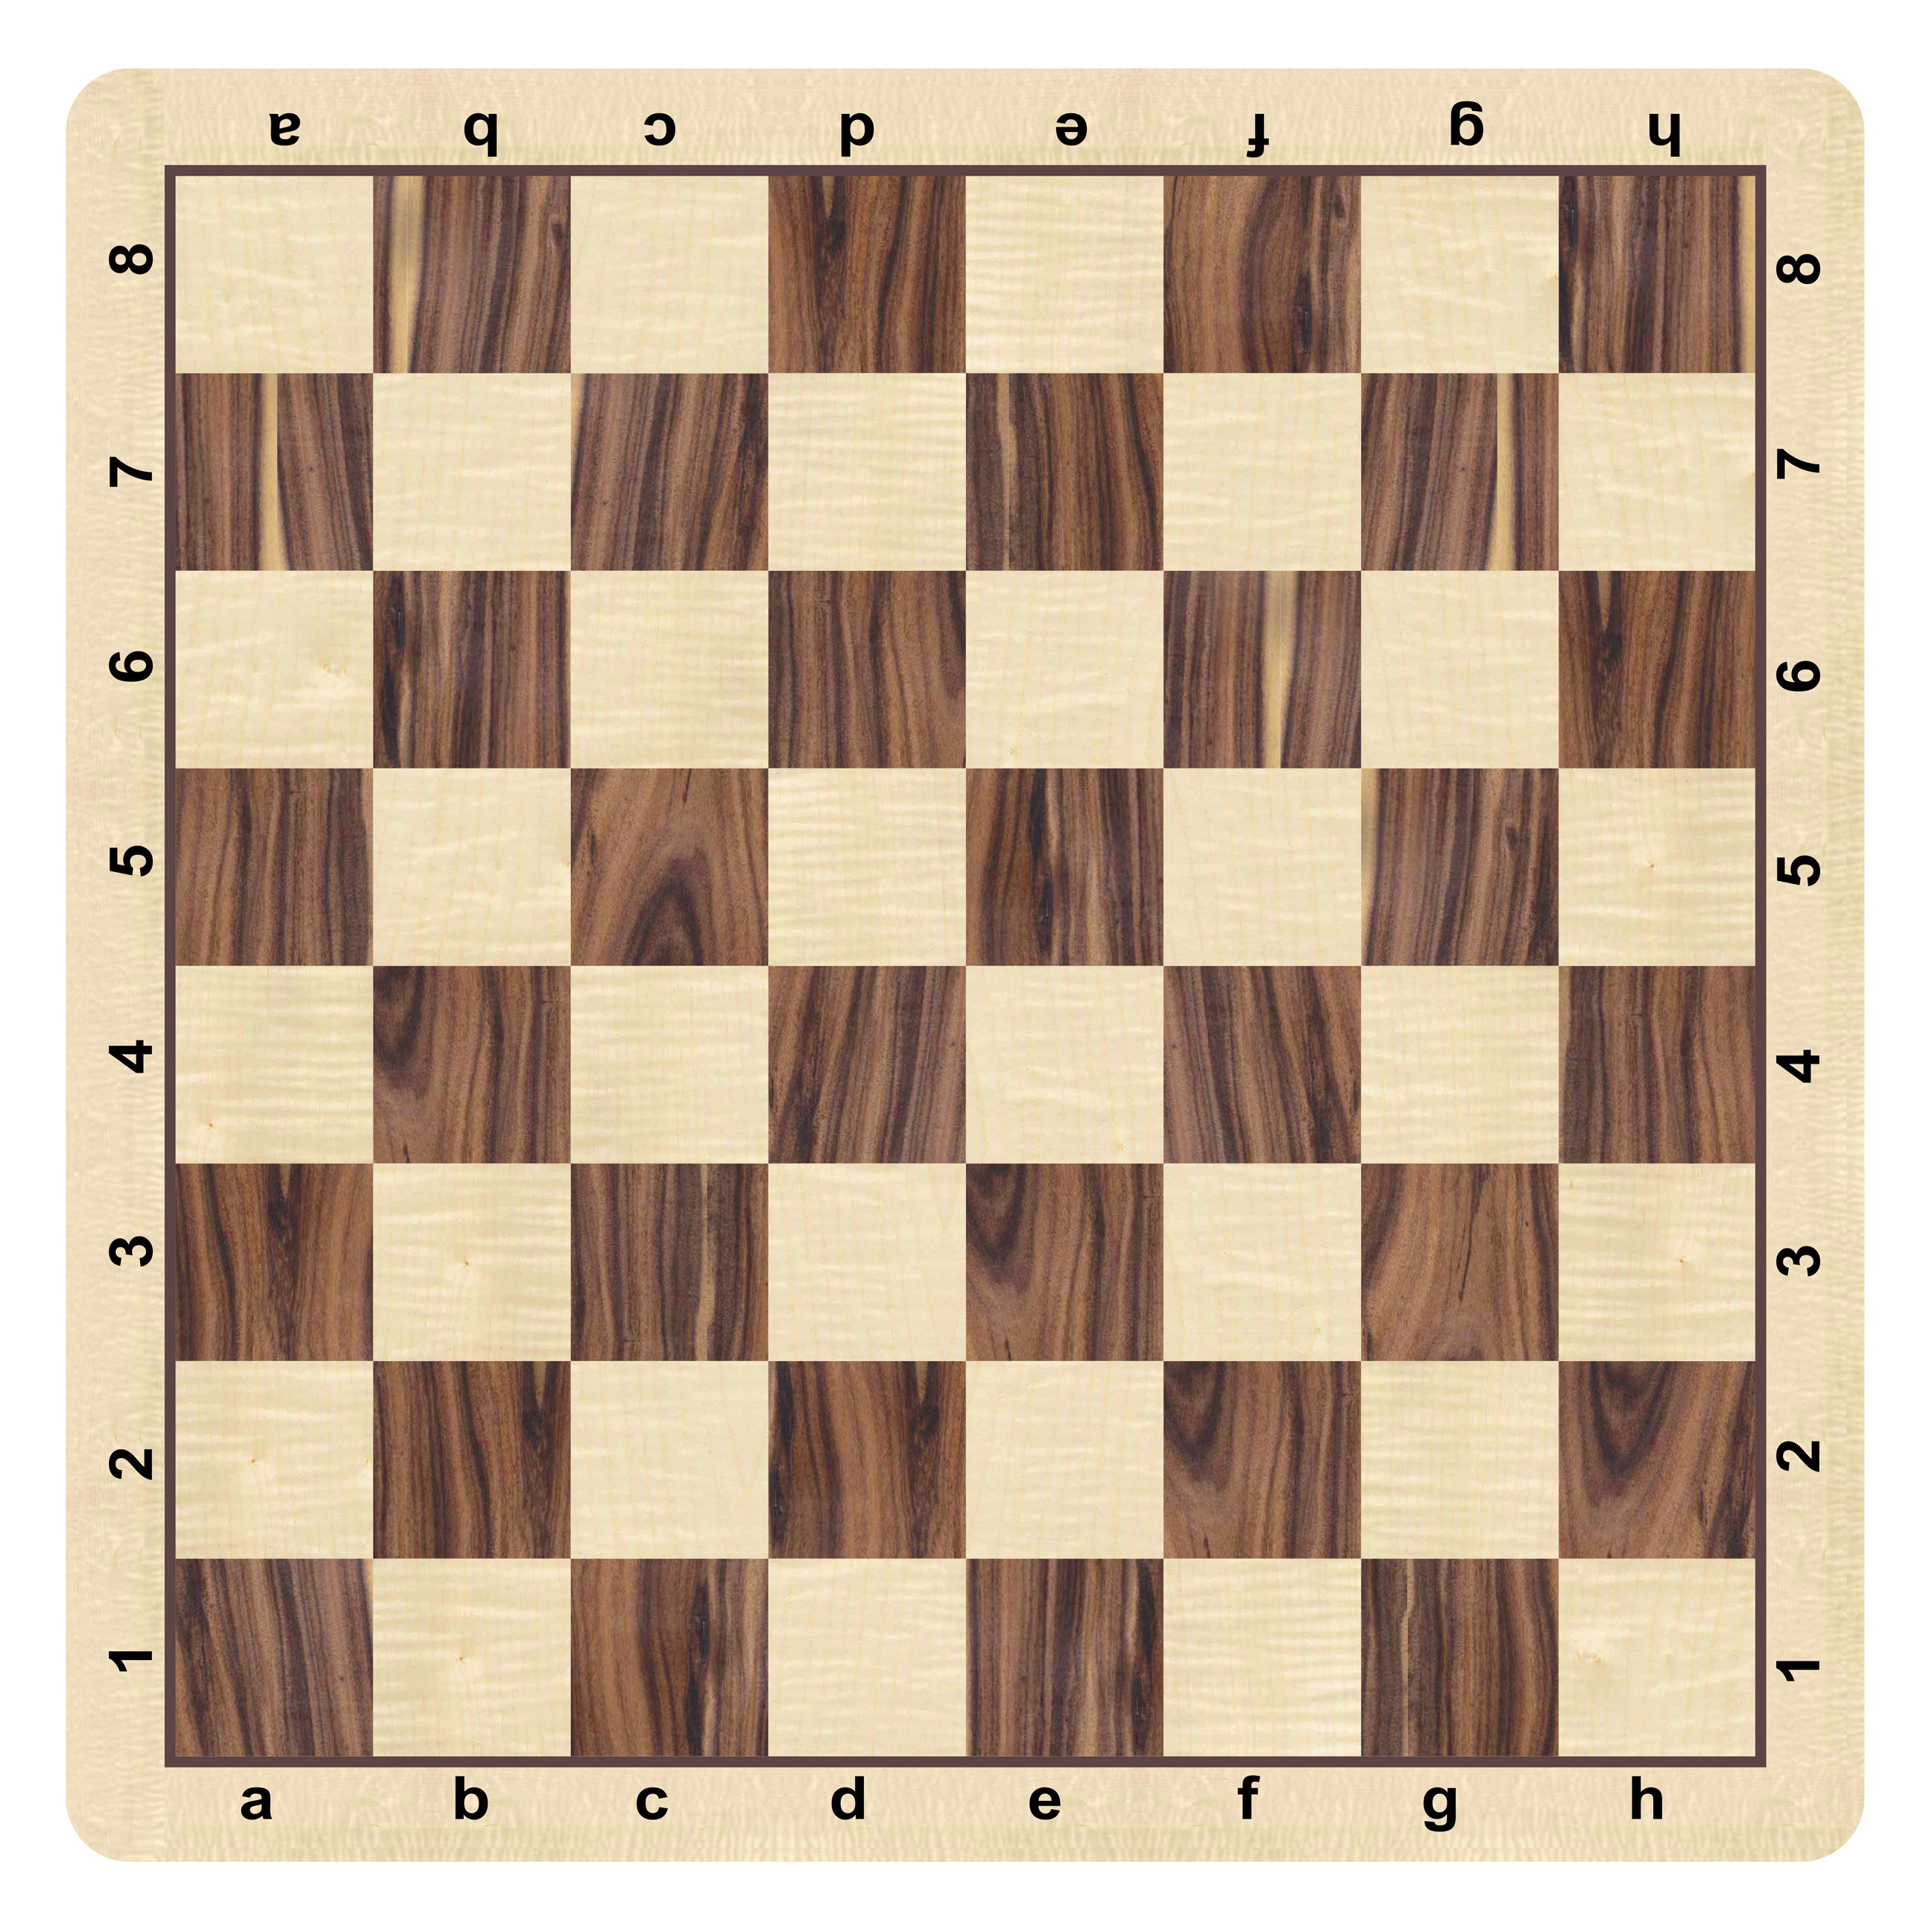
\includegraphics[width=.5\linewidth]{assets/chessboard.jpg}
    \caption{A Standard Chessboard}
    \label{fig:chessboard}
\end{figure}

\end{document}
